%!TEX program = xelatex
\documentclass[UTF8]{article}
%%%引入导言
\usepackage{ctex} 

\usepackage{hyperref}
\usepackage{lastpage}

\usepackage{import}
\usepackage{minted} 
\setminted{encoding=utf-8} 
\usemintedstyle{tango}


\usepackage{media9}
\usepackage{amssymb,amsmath,amsthm,enumerate}
\usepackage[utf8]{inputenc}
\usepackage{array}
\usepackage[parfill]{parskip}
\usepackage{graphicx}
\usepackage{caption}
\usepackage{subcaption}
\usepackage{bm}
\usepackage{amsfonts,amscd}
\usepackage[]{units}
\usepackage{multicol}
\usepackage{multirow}
\usepackage{tcolorbox}
\usepackage{physics}
\usepackage{tikz}

\usepackage{xcolor}

\usepackage{indentfirst}
\setlength{\parindent}{2em} 


\usepackage{pifont}
\newcommand{\cmark}{\ding{51}}
\newcommand{\xmark}{\ding{55}}

\usepackage{algorithm2e}
\renewcommand{\thealgocf}{}

% Glossary entries
\usepackage[acronym]{glossaries}

\newcommand{\empy}[1]{{\color{darkorange}\emph{#1}}}
\newcommand{\empr}[1]{{\color{cardinalred}\emph{#1}}}
\newcommand{\examplebox}[2]{
\begin{tcolorbox}[colframe=darkcardinal,colback=boxgray,title=#1]
#2
\end{tcolorbox}}

\newtcolorbox{mybox}[2][]{colbacktitle=red!10!white, colback=blue!10!white,coltitle=red!70!black, title={#2},fonttitle=\bfseries,#1}


%% Fancy headers and footers
%\headrule
%\firstpageheader{CS242029\\2022年秋}{课后作业 \psetnumber\\\psetdescription}{截止日期\\ \duedate  \duetime 点}
%\runningheader{CS242029}{课后作业 \psetnumber}{\authorname}
%\footer{}{\footnotesize{Page \thepage\ of \pageref{LastPage}}}{}

%% 自定义命令
% =========================================================
%%%% 设置常用字体字号,与MS Word相对应
%% 一号, 1.4倍行距
\newcommand{\yihao}{\fontsize{26pt}{36pt}\selectfont}
%% 二号, 1.25倍行距
\newcommand{\erhao}{\fontsize{22pt}{28pt}\selectfont}
%% 小二, 单倍行距
\newcommand{\xiaoer}{\fontsize{18pt}{18pt}\selectfont}
%% 三号, 1.5倍行距
\newcommand{\sanhao}{\fontsize{16pt}{24pt}\selectfont}
%% 小三, 1.5倍行距
\newcommand{\xiaosan}{\fontsize{15pt}{22pt}\selectfont}
%% 四号, 1.5倍行距
\newcommand{\sihao}{\fontsize{14pt}{21pt}\selectfont}
%% 半四, 1.5倍行距
\newcommand{\bansi}{\fontsize{13pt}{19.5pt}\selectfont}
%% 小四, 1.5倍行距
\newcommand{\xiaosi}{\fontsize{12pt}{18pt}\selectfont}
%% 大五, 单倍行距
\newcommand{\dawu}{\fontsize{11pt}{11pt}\selectfont}
%% 五号, 单倍行距
\newcommand{\wuhao}{\fontsize{10.5pt}{10.5pt}\selectfont}
% =========================================================
\usepackage{geometry}
%%%导言结束

%%%设置设计报告公共信息
%\newcommand*{\Department}{信息工程学院}
\newcommand*{\Department}{计算机与人工智能学院}
\newcommand*{\Course}{《数据结构》}

%%%请修改综合设计报告
\newcommand*{\ProjectName}{计划安排提醒系统}

%%%补充综合设计参与人信息

%%%设置班级、专业和起止时间
\newcommand*{\Class}{}
\newcommand*{\DepAndMajore}{}
\newcommand*{\DateStart}{2022.11.10}
\newcommand*{\DateEnd}{2022.12.1}

%%%正文区
\begin{document}
%%%封面,请不要修改
\begin{titlepage}
  \newgeometry{top=2.5cm, bottom=2.5cm, left=2.cm, right=2.cm}
  \begin{center}
    { \erhao \bf
      \makebox[10cm][s]{\bf \Department}  \\
      \makebox[10cm][s]{\Course 综合设计报告}\\
    }
    \vfill

    \sihao
    \setlength{\baselineskip}{1cm}
    \bf
    \begin{tabular}{cl}
    设计名称:&\underline{\makebox[7cm]{\ProjectName}}\par\\
    小组成员:&\underline{\makebox[7cm]{\MemberOne,\MemberTwo}}\par\\
    &\underline{\makebox[7cm]{\MemberThree,\MemberFour}}\par\\
    &\underline{\makebox[7cm]{\MemberFive}}\par\\
    专业班级:&\underline{\makebox[7cm]{\Class }}\par\\
     \makebox[4em][s]{系(院)}:&\underline{\makebox[7cm]{\DepAndMajore}}\par\\
    设计时间:&\underline{\makebox[7cm]{\DateStart \; -- \; \DateEnd}}\par\\   
    
    \end{tabular}
    \vfill
	\begin{tabular}{|lcccc|}
	\hline
	评价指标 & & \multicolumn{3}{r|}{\multirow{2}{*}{成绩:\underline{\makebox[1.8cm]{}}}}\\	
	&&\multicolumn{3}{r|}{}\\
	1.报告的规范性&【规范】 & 【较规范】&【一般】&【差】\\
	2.程序、算法的规范性&【规范】 & 【较规范】&【一般】&【差】\\
	3.写作思路的清楚性&【清楚】 & 【较清楚】&【一般】&【差】\\
	4.问题描述的清楚性&【清楚】 & 【较清楚】&【一般】&【差】\\
	5.数据结构设计合理性&【合理】 & 【较合理】&【一般】&【差】\\
	6.算法设计的合理性&【合理】 & 【较合理】&【一般】&【差】\\
	7.完成情况 &【好】&【较好】&【一般】&【差】\\
	8.创新性(或新意)&【有】&【无】&&\\ \hline 
	\end{tabular}
  \end{center}
  \centering
  \vfill

\end{titlepage}

\newpage
\restoregeometry
\newpage

\pagenumbering{Roman}
\setcounter{page}{1}
\tableofcontents
\newpage
\setcounter{page}{1}


%%%% 设置为小四号字
\xiaosi

%%%% 建议各讲内容分别存储在一个独立的tex文件中,以便分类编写和管理
\pagenumbering{arabic}
\setcounter{page}{1}
\begin{center}
\bf \sanhao{《数据结构》课程综合设计}
\end{center}

\section{设计目的}
在计算机科学中,数据结构是一般程序设计的基础。通过综合设计,使学生学会分析研究数据结构的特征,以便为应用涉及的数据选择适当的逻辑结构、存储结构及相应的算法,掌握算法的时间复杂度分析技术。另一方面,综合设计也是复杂程序设计的训练过程,要求学生编写的程序结构符合软件工程规范,培养他们的数据抽象能力、建模能力和算法设计能力,提高复杂问题的解决能力,为后续课程的学习和应用奠定基础。

\section{任务与要求}

要求学生以5人一组,自由结合,从给定的综合设计题目中进行选择。本次设计题目是设计内容不固定的题目,这就要求学生自己先确定本组设计题目,然后确定具体内容和设计目标,从而为数据结构设计、数据建模和算法设计奠定基础。提交的资料包含综合设计纸质版、电子版及源程序电子版。


\section{计划安排提醒系统}
\subsection{系统(问题)描述}
在现实生活中,大家都有许多的事情需要处理,并且由于有时候事务繁多,一个计划安排提醒的功能就会让人们能够及时的完成待办的事情。所以我们制作了一个“计划安排提醒系统”。他的主要功能是可以让用户自己添加相关的代办,并选择时间,事件。在这个事件要办理的当天以及前三天均会提醒用户,这很好的避免了用户忘记时间而没有完成相关的日程。
\subsection{任务分配}
我们小组四个人,每个人都在这个系统制作中是不可或缺的一部分。\\
1.小组长,主要负责事务分配,链表的构建以及相应添加,删除功能等函数的实现,以及文件读写和解决在制作过程中产生的一些bug。

2.主要负责EasyX可视化部分的设计以及与链表功能的对接。并且实现了与现实时间比较的函数,并且在改进代码的功能过程中贡献了很大的力量。

3.主要负责链表数据的处理,比如时间的排序,以及数据的修改等函数的编写,也写出了计算页数的函数,给EasyX的页数计算提供了一定的基础。

4.主要负责日程提醒界面的设计以及修改,分别对三天前提醒以及当日提醒的功能编写了相关的函数。

对于课程设计文档的编写,是由我们四个人分工进行的,每个人编写自己熟悉的部分,并且作业量都差不多。\\
在任务分配的过程中,我们主要考虑每个人拿手的技能,以及任务分配的平均性,来合理的分配任务,以此来保证每个人都能够参与到课程设计中来,并且在课程设计过程中学到新的知识,巩固旧的知识。
\subsection{系统需求}
1.具备添加日程安排的功能,其中需要添加的内容有日程的时间,以及日程的内容。

2.具备删除日程安排的功能,其中删除功能具体到程序中应该体现为两个方面,分别是完成了日程,以及针对错误日程或者想要取消日程的删除。

3.具备修改日程安排的功能,因为数据内容的特殊性,要求能够结合实际合理地实现该功能。

4.拥有提醒功能,能对用户尚未完成的日程进行判断,若当日有待办事项,应该提醒用户;若有临近日程,例如三日后的日程,也应该提醒用户;若今日无待办事项,也应当提醒用户,以便用户清楚自己的日程。

5.能够以合理的形式显示安排中的日程,使用户对于自己的行程能够一目了然。

\subsection{设计思想}
本系统以用户体验为核心,将用户的使用感受放在第一位,选用更为用户接受的图形化界面,将一切复杂的数据以合理美观的形式显示在用户眼前,同时根据日程数据特殊的形式以及需要频繁地查改以及数据数目的不确定性等的特点,本系统选用链表结构实现对数据的存储和操作;在开发过程中,我们针对本系统体量较小的特点,采用合作开发模式,将软件需求模块化后分别进行代码的编写,最后将数据操作以及UI模块进行整合,形成完整的程序。
\subsubsection{数据结构的选择和设计}
数据结构:链表,链表中的数据采用的是结构体类型的数据
\begin{minted}{C}
#include<stdio.h>
//定义链表所存数据 
typedef struct Content
{
    char thing[100];
    char time[15]={0};
    bool preReming;
}content;
//定义链表节点
typedef struct ThingNode
{
    content data;
    struct ThingNode* next;
    int length;
}List;
//创建链表
List* creat_list()
{
    List* node = (List*)malloc(sizeof(List));
    node->next = NULL;
    node->length = 0;
    return node;
}
\end{minted}
采用链表来储存日程的相关数据,主要是因为各个日程之间没有什么相关性,单个独立,并且采用链式存储查找与删除都十分方便。采用链表可以更加高效的储存数据\\
\subsubsection{算法设计}

1.冒泡排序算法:是一种稳定排序算法,通过冒泡排序算法,稍微根据数据的类型进行了一定的修改,将日程的时间作为关键字,对日程进行排序。使日程更加的有序,便于查看
\begin{minted}{C}
void ThingSort_ByTime(List* head) {
//按照日期从早到晚排序
//采用冒泡法进行排序
List* front, * middle , * rear;
for (int i = 0; i < head->length - 1; i++) {
    front = head, middle = head->next, rear = middle->next;
     for (int j = 0; j < head->length - 1 - i; j++) {
         if (strcmp(middle->data.time, rear->data.time) > 0) {
            middle->next = rear->next;
            rear->next = middle;
            front->next = rear;  }
            front = front->next;
            middle = front->next;
            rear = middle->next; }
    }
}
\end{minted}
2.链表操作的算法:比如修改日程根据链表数据的修改进行,由于这个链表数据内容较多,所以采用逐个输入的办法,通过EasyX来进行可视化,通过按钮等函数来进行可视化交互。还有链表数据的插入,删除等。\\
3.UI算法:在修改日程,以及日程已完成之后可以点击日程行后边的按钮,来完成上述操作。通过EasyX函数库,根据鼠标位置同时结合位置来判断数据在链表中的位置,来对该数据进行操作。其他的UI操作还有“按钮”,“弹出界面”等。
\begin{minted}{c}
void things_finish(ExMessage msg)
{
int i = 35, j = 0;
for (j; j < 15; j++) {
if (msg.x >= 1030 && msg.y >= 140 + i * j && msg.x <= 1080 && msg.y <= 170 + i * j) {
    clearroundrect(1032, 140 + i * j, 1080, 171 + i * j, 0, 0);
    button_delete(1032, 142 + i * j, 1078, 169 + i * j, "已完成", YELLOW, skyblue);
    if (msg.message == WM_LBUTTONDOWN) {
        delete_list(ThingList, j+1, page_cnt);
        show_things();}
        }
    else {
        button_delete(1032, 140 + i * j, 1080, 171 + i * j, "", YELLOW, gray);}
         }
    write_file(ThingList, "thing.txt");
}
\end{minted}
4.翻页算法:根据链表长度将数据分页,更加清楚的展示日程。根据数据选择的页面刷新显示相应的页面。\\
5.time函数算法:通过对时间的英文首字母比对,将时间存放在Temp数组中,并最后将Temp数组转化为字符串。
\subsection{实现细节说明}
系统的关键算法可分为三个部分:数据的读取、界面的排版、数据的处理及结果反馈

\subsubsection{数据的读取}

运用链表,便于增删修改。其中,用头插法实现数据的增加,并用冒泡排序来确定新增数据的插入位置。

1.头插法:
\begin{minted}{c}
//添加日程(头插法)
void add_list(List*& head, Content data)
{
    List* node = creat_list();
    node->data = data;
    node->next = head->next;
    head->next = node;
    head->length++;
}
\end{minted}
2.冒泡排序
\begin{minted}{c}
void ThingSort_ByTime(List* head) {
    //按照日期从早到晚排序
    //采用冒泡法进行排序
    List* front, * middle , * rear;
    for (int i = 0; i < head->length - 1; i++) {
        front = head, middle = head->next, rear = middle->next;
        for (int j = 0; j < head->length - 1 - i; j++) {
            if (strcmp(middle->data.time, rear->data.time) > 0) {
                middle->next = rear->next;
                rear->next = middle;
                front->next = rear;
            }
                front = front->next;
                middle = front->next;
                rear = middle->next;
        }
    }
}
\end{minted}
排序后的日程如下图所示:\\
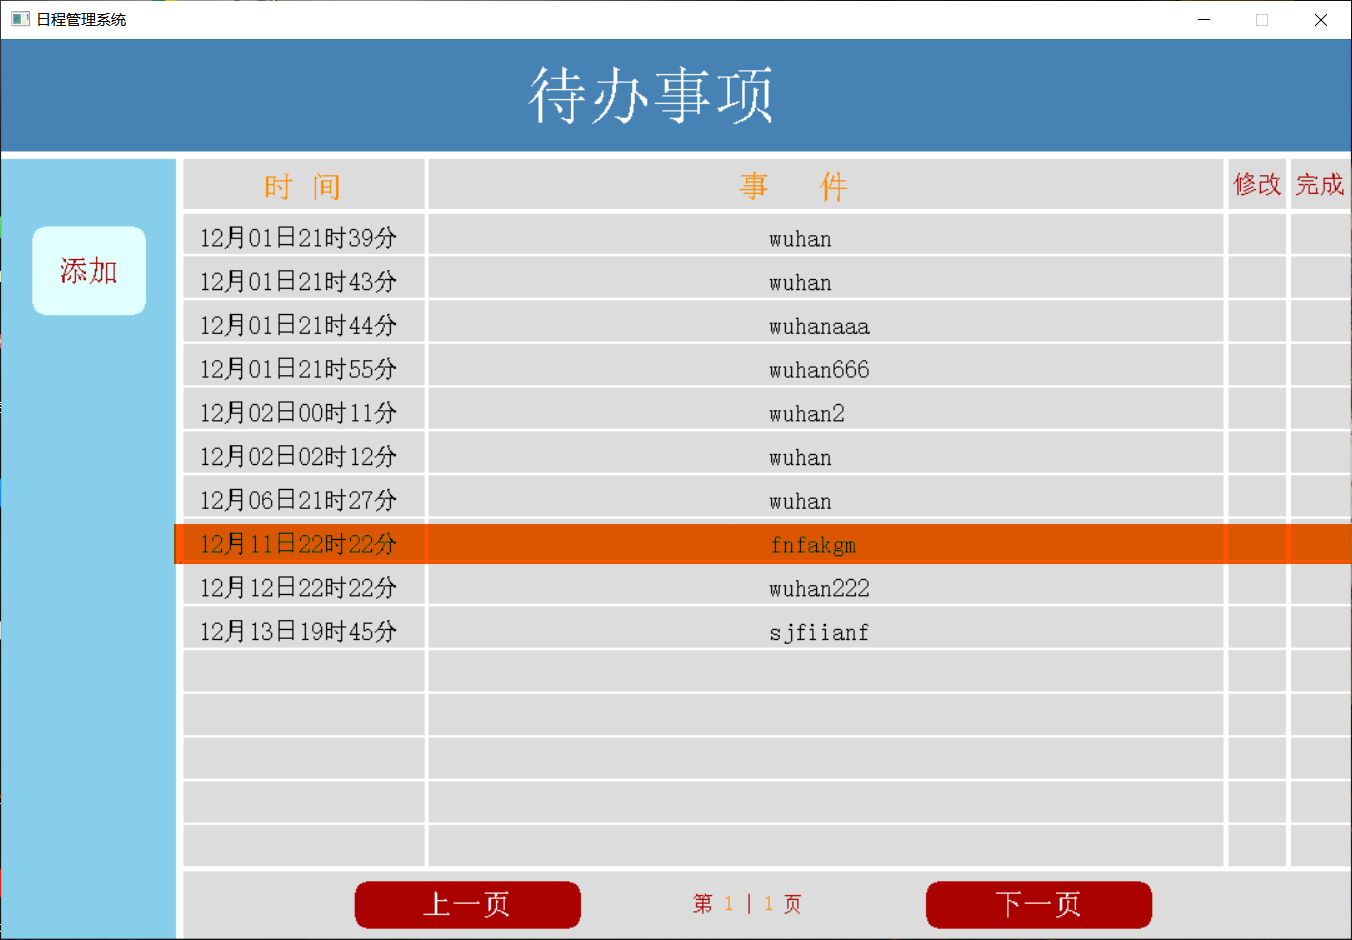
\includegraphics[width=.8\textwidth]{1.1.png}

\subsubsection{界面的排版}

应用easyx来进行界面设计的大部分内容,例如界面的长宽、背景颜色、字体大小颜色、按键的大小和颜色等。(以下以系统首页为例)

1.界面的长宽:
\begin{minted}{c}
initgraph(500, 500);
\end{minted}

2.背景颜色:
\begin{minted}{c}
setbkcolor(RGB(225, 245, 245));
\end{minted}

3.字体大小颜色:
\begin{minted}{c}
settextcolor(RGB(225, 0, 245));
settextstyle(24, 0, "宋体");
outtextxy(175, 150, "今日无待办事项");
\end{minted}

4.按键大小颜色:
\begin{minted}{c}
//按钮函数
void button(int left, int top, int right, int bottom,
    const char* flag, COLORREF word, COLORREF back)
{
    int x, y;
    settextcolor(word);
    setfillcolor(back);
    setbkmode(TRANSPARENT);
    settextstyle(24, 0, "宋体");
    solidroundrect(left, top, right, bottom, 20, 20);
    x = left + (right - left - textwidth(flag)) / 2;
    y = top + (bottom - top - textheight(flag)) / 2;
    outtextxy(x, y, flag);
}
\end{minted}

5.鼠标对界面的控制:
\begin{minted}{c}
ExMessage msg;
peekmessage(&msg, EM_MOUSE);
if (msg.x >= 210 && msg.y >= 300 && msg.x <= 290 && msg.y <= 350) {
    clearroundrect(210, 300, 290, 350, 20, 20);
    button(210, 300, 290, 350, "好的", dark_orign, RED);
    if (msg.message == WM_LBUTTONDOWN) {
        break;
    }
}
else {
    button(210, 300, 290, 350, "好的", dark_orign, skyblue);
}
\end{minted}
日程提醒界面图示:

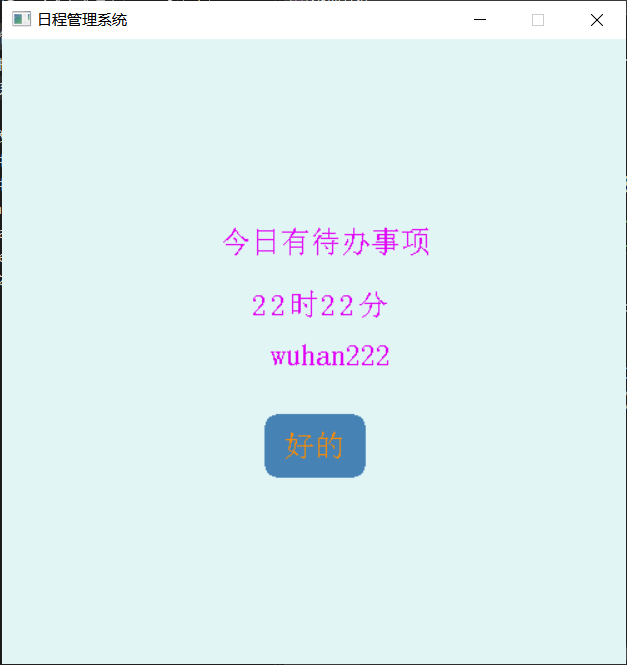
\includegraphics[width=.5\textwidth]{2.1.png}

\subsubsection{数据的处理及结果反馈}
1.本机时间的读取:

具体使用time函数,获取本机时间并转化为标准格式。因程序进行运算时使用的是字符串,所以再通过ReadNowTime函数中部分代码实现了从标准格式到字符串的转换。

本机时间的读取和转换:
\begin{minted}{c}
#include<windows.h>
time_t rawtime;
struct tm* timeinfo;
time(&rawtime);
timeinfo = localtime(&rawtime);
\end{minted}
2.提醒时间的判断:

系统共有两个提醒时间,一为当天,二为提前三天,其中判断当天与否只需比较列表中的字符串与当前时间的字符串中前八位字符是否相同即可;提前三天的需要进行字符串的拆分比较,期间需要考虑年份月份等问题。

\subsection{测试数据及测试结果}
\subsubsection{当天提醒}
输入样例:

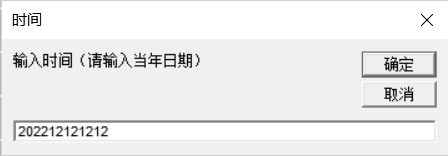
\includegraphics[width=.5\textwidth]{4.0.png}

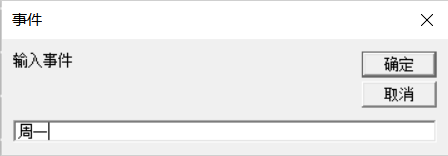
\includegraphics[width=.5\textwidth]{4.0.1.png}

输出样例:

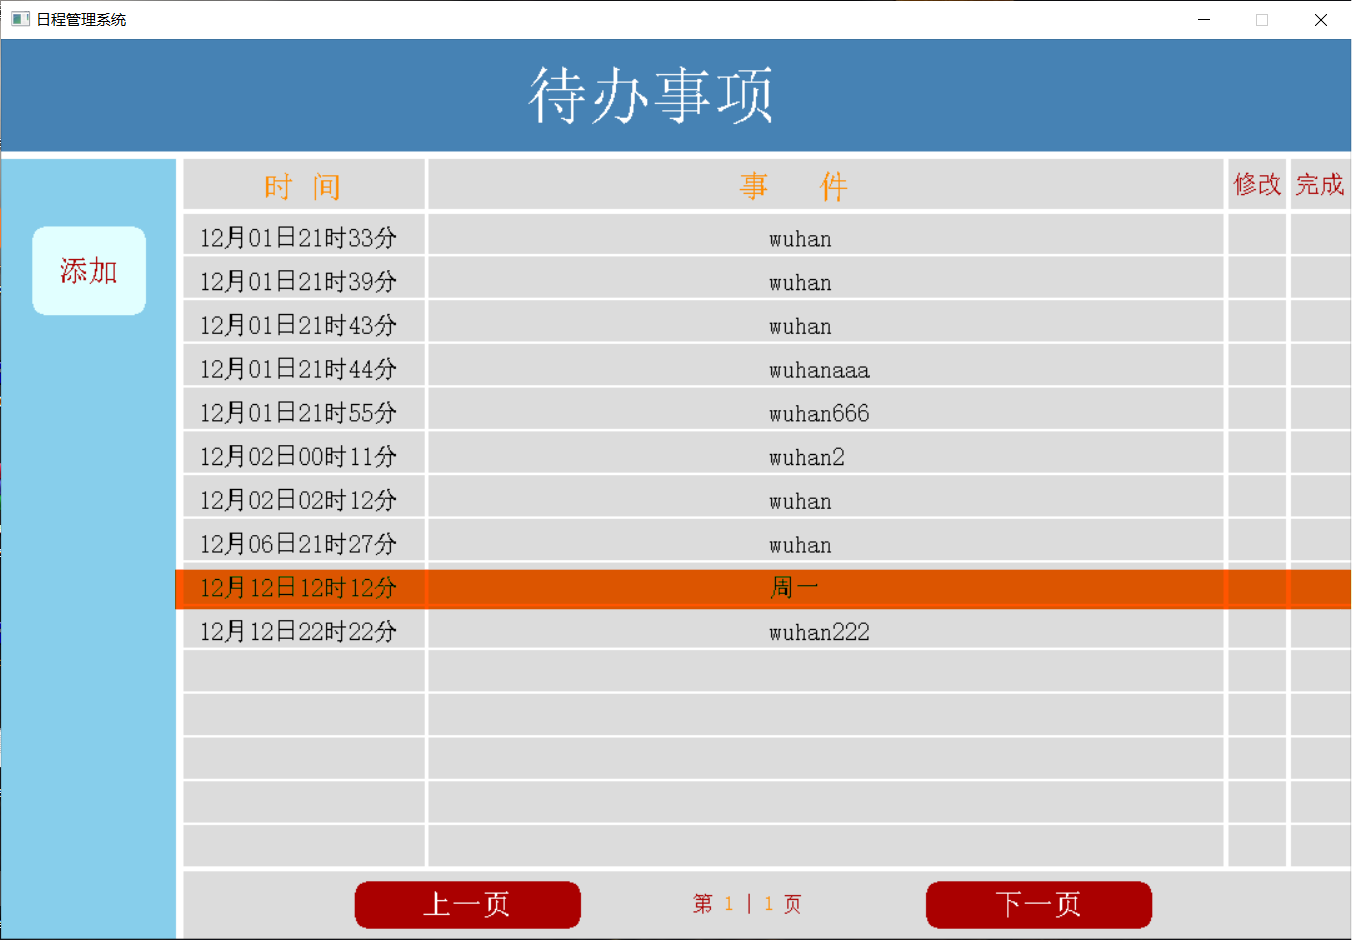
\includegraphics[width=.8\textwidth]{4.1.0.png}

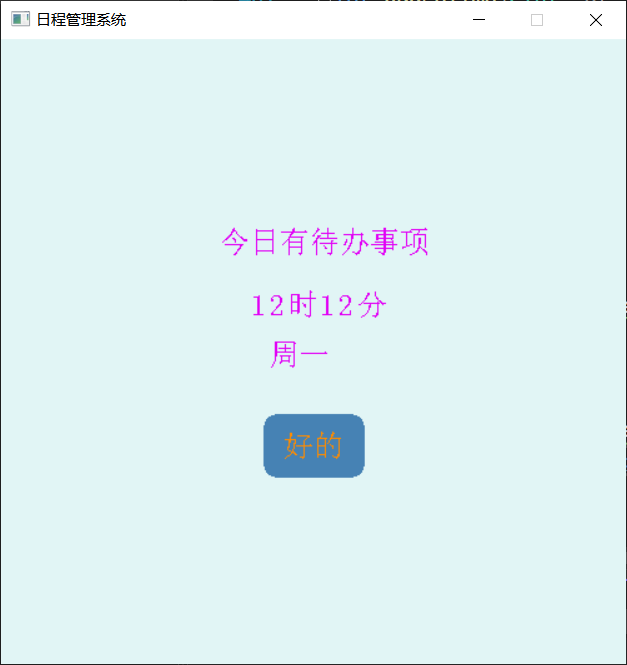
\includegraphics[width=.5\textwidth]{4.1.png}

\subsubsection{提前三天提醒}
输入样例:

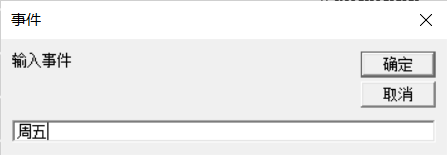
\includegraphics[width=.5\textwidth]{4.2.1.png}

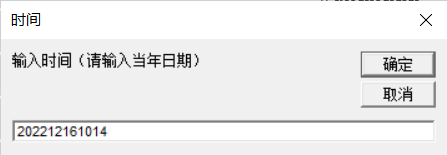
\includegraphics[width=.5\textwidth]{4.2.2.png}

输出样例:

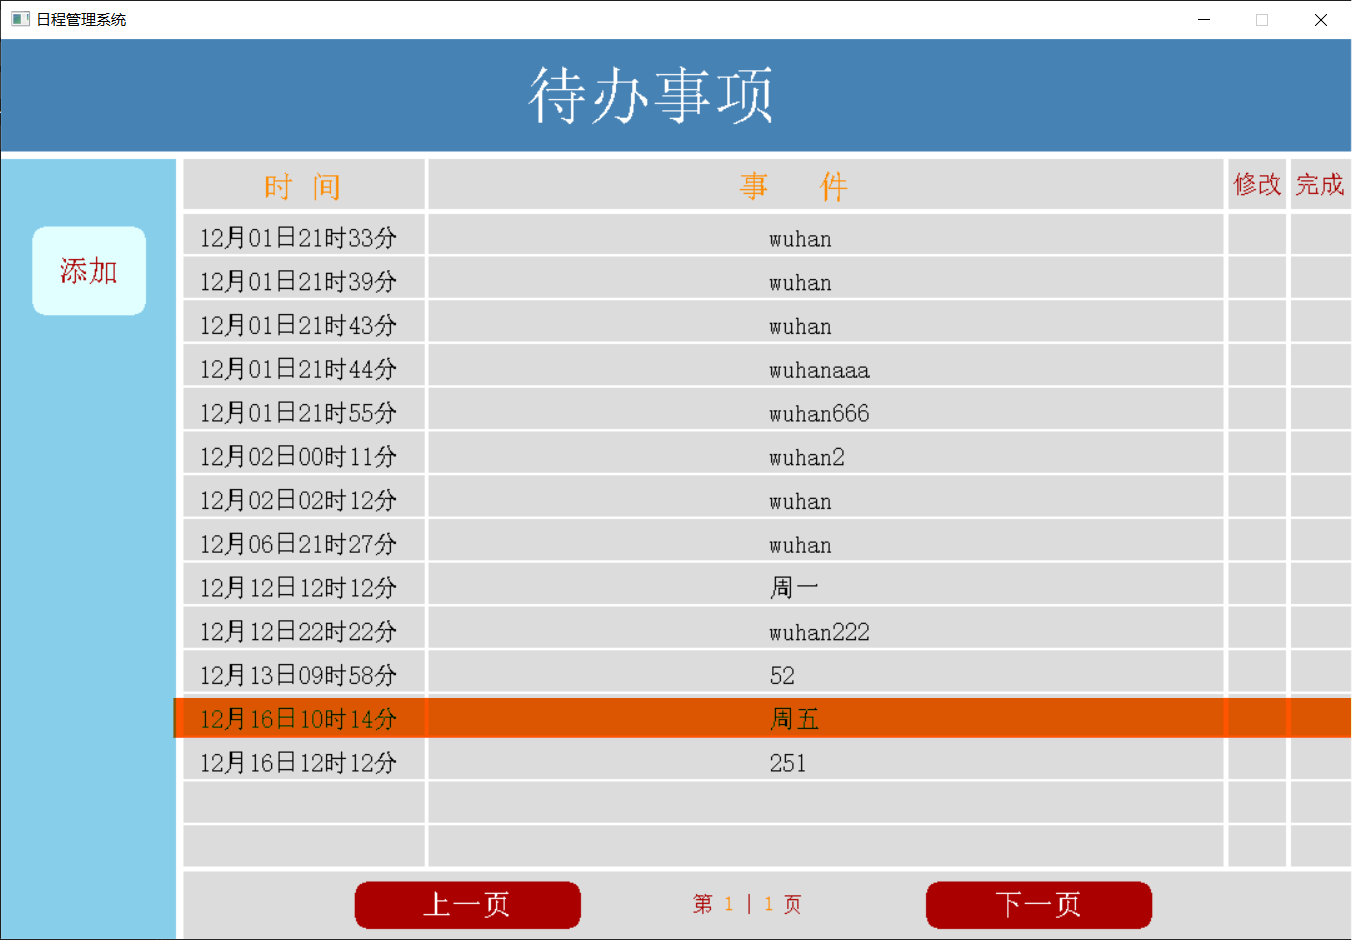
\includegraphics[width=.8\textwidth]{4.2.3.png}

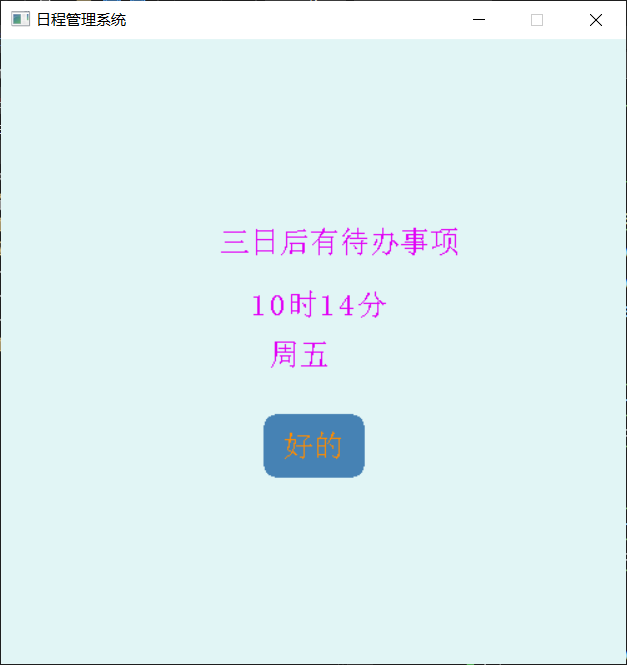
\includegraphics[width=.5\textwidth]{4.2.4.png}

\section{总结}
\subsection{系统特点及创新}
本系统采用EasyX图形库,来达到页面可视化的效果。通过使用EasyX所包含的头文件graphics.h来绘制页面窗口及按钮,另外使用time.h头文件,读取计算机现在的时间,从而与用户输入的时间相比较来判断是否达到用户设置的提醒时间,此外,用户还可以选择是否需要提前三天进行提醒。用户可以首先输入乱序的所有需要提醒的事项,然后可以进行一键根据输入的时间自动进行对事件依据时间进行排序。

\subsection{遇到的问题及解决思路}
遇到的困难1:如何对用户输入的所有事件根据其事件进行排序,因为在创建链表用以存储用户输入数据时,为创建的单链表,解决方案初始化了三个指针,用以指示待删除结点的头结点、待删除结点和待删除结点的下一节点,在删除结点后,第一指针直接指向第三指针。

遇到的困难2:时间表示的选择问题,在程序内的时间可以是预置时间也可以和本计算机的时间一致,在时间的选择上我们选择了使用time.h头文件使程序内时间为本计算机时间。

遇到的困难3:在事件的选择上,我们本想使用音乐播放函数,使事件达到用户指定时间时播放音乐以提醒用户,但由于该程序并不是一直运行,只在用户打开本程序时运行,所以我们将提醒方式改为在某一天需要所的事情,而并非是在该做事情的时间提醒。

遇到的困难4:多人项目合作难以及多人合作变量问题。由于小组每个人的编程习惯并不相同,因此在各个任务程序的协调性上存在难题,最终经过不断的交流和沟通,对各部分代码的讨论和修改我们最终解决了这些困难。

遇到的困难5:代码注释,为了使设计不同功能的同学间可以相互调用功能函数,代码注释是必要的。解决的方法是,每位同学在编写代码时尽量做到每个功能所用的方法和每部分代码作用给予注释,同时,必要的注释也为我们减少了不必要的交流沟通,从而提高了编程和调试的效率。

\bibliographystyle{plain}
\bibliography{Report}
\end{document}

%%% Local Variables:
%%% mode: latex
%%% TeX-command-extra-options: "-shell-escape"
%%% TeX-master: t
%%% TeX-engine: xetex
%%% End: